\documentclass[10pt,a4paper]{article}
\usepackage[margin=2cm]{geometry}
\usepackage{amsmath,amssymb}
\usepackage{booktabs,array,tabularx}
\usepackage{xcolor}
\usepackage{xurl}
\usepackage[hidelinks]{hyperref}
\usepackage{enumitem}
\usepackage{graphicx,float,caption}
\captionsetup{font=small,labelfont=bf}
\setlist{itemsep=1pt,topsep=3pt}
\newcolumntype{L}{>{\raggedright\arraybackslash}X}
\setlength{\parindent}{0pt}\setlength{\parskip}{4pt}
\title{\textbf{Tech note: A1 data/sim robustness, round 3 (V-plane normalisation and cross-domain pretraining)}}
\author{}
\date{}
\begin{document}
\maketitle
\vspace{-3em}
Date: 2026-11-23. Part 1 is inference only; Part 2 trains 4 new backbones and 24 downstream runs.

Plans:

\begin{itemize}
\item \texttt{docs/\allowbreak{}a1\_\allowbreak{}check\_\allowbreak{}round\_\allowbreak{}3\_\allowbreak{}preplan.md} (requests)
\item \texttt{docs/\allowbreak{}a1\_\allowbreak{}check\_\allowbreak{}round\_\allowbreak{}3\_\allowbreak{}plan.md} (implementation plan)
\end{itemize}
Raw outputs: \texttt{fm4npp-lartpc-work/\allowbreak{}a1r3/\allowbreak{}}

\begin{itemize}
\item \texttt{novnorm/\allowbreak{}summary.md} (Part 1)
\item \texttt{summary.md}, \texttt{summary.json} (Part 2)
\item \texttt{pre/\allowbreak{}}, \texttt{down/\allowbreak{}}, \texttt{eval/\allowbreak{}} (per-run outputs)
\item \texttt{STATUS} (job log)
\end{itemize}
\textbf{Rerun note.} \texttt{cl\_\allowbreak{}sim2real\_\allowbreak{}finetune\_\allowbreak{}s1} and \texttt{cl\_\allowbreak{}real2sim\_\allowbreak{}finetune\_\allowbreak{}s0} were each run twice concurrently by a job-queue lock race (fixed afterwards). Both were rerun on 2026-11-23 and all numbers below use the rerun results. The earlier outputs are kept in \texttt{fm4npp-lartpc-work/\allowbreak{}a1r3/\allowbreak{}quarantine\_\allowbreak{}race\_\allowbreak{}20261123/\allowbreak{}}. Real-domain T1 charge-weighted, old $\rightarrow$ new: \texttt{cl\_\allowbreak{}sim2real\_\allowbreak{}finetune\_\allowbreak{}s1} 0.9219 $\rightarrow$ 0.9214; \texttt{cl\_\allowbreak{}real2sim\_\allowbreak{}finetune\_\allowbreak{}s0} 0.6484 $\rightarrow$ 0.6681.

\section*{Summary}
\textbf{Part 1: \texttt{w\_\allowbreak{}meas3d\_\allowbreak{}noVnorm} (V-plane table not renormalised at the anode).}

\begin{itemize}
\item \textbf{The un-normalised V table is harsher for both models.}
\begin{itemize}
\item \textbf{CL:} T1 charge-weighted $-$0.421 (against $-$0.288 for \texttt{w\_\allowbreak{}meas3d}), per-event median $-$0.540 (against $-$0.328), T2 $-$0.087 (against $-$0.055).
\item \textbf{C + XF:} T1 charge-weighted $-$0.058 (against $-$0.038), per-event median $-$0.075 (against $-$0.046), T2 $-$0.005 (against $-$0.004).
\end{itemize}
\item \textbf{The extra damage is in the V plane.} V alone with the un-normalised table costs CL $-$0.112 in T1 ($-$0.025 normalised) and C + XF $-$0.028 ($-$0.006 normalised). The V-plane T1 for CL falls by $-$0.50 (all planes together).
\end{itemize}
\textbf{Part 2: cross-domain pretrain $\rightarrow$ downstream.} Sim is the unaltered open data. Real is the \texttt{w\_\allowbreak{}meas3d} hit widths on simulated-$\nu$ hits plus \texttt{l\_\allowbreak{}comb80} light. Real-domain T1 and T2 are the primary results.

\begin{itemize}
\item \textbf{The downstream domain sets the real-domain score for finetuned models.} CL finetuned with real downstream labels reaches T1 charge-weighted 0.9175 when pretrained on real and 0.9214 when pretrained on sim. The existing sim-only CL models score 0.621 on the same real data, and sim $\rightarrow$ sim retrained on the disjoint lists scores 0.598. C + XF is 0.881 (real $\rightarrow$ real), 0.829 (sim $\rightarrow$ real) and 0.808 (existing).
\item \textbf{Pretraining domain matters more when frozen.} CL frozen, real-domain T1: real $\rightarrow$ real 0.893, sim $\rightarrow$ real 0.845, real $\rightarrow$ sim 0.763, sim $\rightarrow$ sim 0.496. Real-domain pretraining gives a frozen CL backbone most of the robustness that finetuning otherwise provides.
\item \textbf{CL beats C + XF in-domain; C + XF is less sensitive to the shift.} Finetuned real $\rightarrow$ real: CL 0.9175, C + XF 0.8813. Finetuned arms with a sim downstream domain lose 0.26--0.33 in T1 (CL) and 0.05--0.10 (C + XF) when evaluated on the real domain instead of the sim domain.
\item \textbf{Reproduction:} the new sim $\rightarrow$ sim runs (disjoint event lists, re-pretrained) reproduce the existing models on the sim domain within 0.007 in T1 charge-weighted and 0.003 in T2 (all events), in all four model/mode combinations.
\item T2 on all events is 0.93--0.997 everywhere. The bright-subset T2 separates the arms more, but T1 is the main discriminator.
\end{itemize}
\section{Setup}
\begin{itemize}
\item \textbf{Models:} qlfm-M CL (light-in-encoder pretraining, \texttt{--late-light 0}) and qlfm-M C + XF (charge-only pretraining, light added late by cross-attention, \texttt{--late-light 2}).
\item \textbf{Metrics:} same definitions as round 2.
\begin{itemize}
\item \textbf{T1:} $\nu$/cosmic hit F1, charge-weighted (in-run score) and per-event median (paper definition).
\item \textbf{T2:} $\nu$-event AUC, all events and the bright subset (native 3--6 $\mu$s PE $\geq$ 200; this is not the paper \texttt{truth.npz} 200-PE cut).
\end{itemize}
\item \textbf{Scope:} only T1 and T2 are reported. Energy and light (T5) test scores are not reported; the T5 targets stay native in the real-domain downstream runs.
\item \textbf{Uncertainties:} mean $\pm$ seed SD (ddof = 1) over the seeds present. A single seed shows SD 0.0000, which is not an uncertainty. Part 2 has two downstream seeds per arm and one for controls. Per-run bootstrap CIs are in \texttt{summary.md}. Per-seed values are in Appendix A.
\item \textbf{Validation:} Stage 0 gates all passed (tests, splits, pretrain smoke with real/sim throughput ratio 0.983, downstream smoke with no double perturbation, \texttt{qsub}/\texttt{qdel} from a compute node, and Gate 5: \texttt{w\_\allowbreak{}meas3d} reproduces round 2 on all 6 models within 0.002 in T1 and 0.001 in T2).
\end{itemize}
\section{Part 1: \texttt{w\_\allowbreak{}meas3d\_\allowbreak{}noVnorm}}
\subsection{Variants}
In the round-2 \texttt{F\_\allowbreak{}MEAS\_\allowbreak{}3D} table, the V factors were normalised to 1.0 at the anode, but the measured V ratio never reaches 1. The new table keeps Y and U unchanged and leaves V un-normalised (0.900 at the first drift bin):

\begin{center}\small
\setlength{\tabcolsep}{3pt}\renewcommand{\arraystretch}{1.15}
\begin{tabularx}{\linewidth}{LLL}
\toprule
\textbf{Plane} & \textbf{Factors, \texttt{w\_\allowbreak{}meas3d}} & \textbf{Factors, \texttt{w\_\allowbreak{}meas3d\_\allowbreak{}noVnorm}} \\
\midrule
Y & 1.000, 0.967, 0.941, 0.926, 0.915, 0.903 & unchanged \\
V & 1.000, 0.980, 0.954, 0.938, 0.942, 0.941 & 0.900, 0.882, 0.859, 0.844, 0.848, 0.847 \\
U & 1.000, 0.960, 0.922, 0.907, 0.892, 0.880 & unchanged \\
\bottomrule
\end{tabularx}
\end{center}
\begin{center}\small
\setlength{\tabcolsep}{3pt}\renewcommand{\arraystretch}{1.15}
\begin{tabularx}{\linewidth}{LL}
\toprule
\textbf{Variant} & \textbf{Definition} \\
\midrule
\texttt{w\_\allowbreak{}meas3d} & round-2 3D table, all planes \\
\texttt{w\_\allowbreak{}meas3d\_\allowbreak{}noVnorm} & un-normalised V table, all planes \\
\texttt{w\_\allowbreak{}meas3d\_\allowbreak{}V} & normalised V table on V only (f = 1 on U, Y) \\
\texttt{w\_\allowbreak{}meas3d\_\allowbreak{}noVnorm\_\allowbreak{}V} & un-normalised V table on V only \\
\bottomrule
\end{tabularx}
\end{center}
All variants act on simulated-$\nu$ hits only, applied to the 6 existing multi-task models (seeds 0, 1, 2) at inference time.

\subsection{Results ($\Delta$ vs nominal; nominal = absolute)}
Mean $\pm$ seed SD over 3 seeds.

\textbf{qlfm-M CL}

\begin{center}\footnotesize
\setlength{\tabcolsep}{3pt}\renewcommand{\arraystretch}{1.15}
\begin{tabularx}{\linewidth}{LLLLL}
\toprule
\textbf{Variant} & \textbf{T1 charge-wtd} & \textbf{T1 evt-median} & \textbf{T2 all} & \textbf{T2 bright} \\
\midrule
nominal & 0.9185 $\pm$ 0.0002 & 0.9217 $\pm$ 0.0006 & 0.9932 $\pm$ 0.0028 & 0.9882 $\pm$ 0.0035 \\
\texttt{w\_\allowbreak{}meas3d} & $-$0.2877 $\pm$ 0.0165 & $-$0.3280 $\pm$ 0.0199 & $-$0.0554 $\pm$ 0.0082 & $-$0.0778 $\pm$ 0.0196 \\
\texttt{w\_\allowbreak{}meas3d\_\allowbreak{}noVnorm} & \textbf{$-$0.4211 $\pm$ 0.0170} & \textbf{$-$0.5395 $\pm$ 0.0263} & \textbf{$-$0.0868 $\pm$ 0.0111} & \textbf{$-$0.1218 $\pm$ 0.0282} \\
\texttt{w\_\allowbreak{}meas3d\_\allowbreak{}V} & $-$0.0248 $\pm$ 0.0027 & $-$0.0266 $\pm$ 0.0029 & $-$0.0016 $\pm$ 0.0009 & $-$0.0025 $\pm$ 0.0011 \\
\texttt{w\_\allowbreak{}meas3d\_\allowbreak{}noVnorm\_\allowbreak{}V} & $-$0.1122 $\pm$ 0.0033 & $-$0.1317 $\pm$ 0.0015 & $-$0.0042 $\pm$ 0.0023 & $-$0.0069 $\pm$ 0.0037 \\
\bottomrule
\end{tabularx}
\end{center}
noVnorm $-$ \texttt{w\_\allowbreak{}meas3d} (all planes): T1 charge-weighted $-$0.1334 $\pm$ 0.0054, T2 $-$0.0314 $\pm$ 0.0032. V-only, noVnorm $-$ normalised: T1 $-$0.0874 $\pm$ 0.0030, T2 $-$0.0025 $\pm$ 0.0014.

\textbf{qlfm-M C + XF}

\begin{center}\footnotesize
\setlength{\tabcolsep}{3pt}\renewcommand{\arraystretch}{1.15}
\begin{tabularx}{\linewidth}{LLLLL}
\toprule
\textbf{Variant} & \textbf{T1 charge-wtd} & \textbf{T1 evt-median} & \textbf{T2 all} & \textbf{T2 bright} \\
\midrule
nominal & 0.8593 $\pm$ 0.0017 & 0.8621 $\pm$ 0.0017 & 0.9899 $\pm$ 0.0005 & 0.9689 $\pm$ 0.0004 \\
\texttt{w\_\allowbreak{}meas3d} & $-$0.0375 $\pm$ 0.0030 & $-$0.0457 $\pm$ 0.0039 & $-$0.0035 $\pm$ 0.0003 & $-$0.0090 $\pm$ 0.0006 \\
\texttt{w\_\allowbreak{}meas3d\_\allowbreak{}noVnorm} & \textbf{$-$0.0579 $\pm$ 0.0036} & \textbf{$-$0.0751 $\pm$ 0.0040} & \textbf{$-$0.0053 $\pm$ 0.0002} & \textbf{$-$0.0136 $\pm$ 0.0014} \\
\texttt{w\_\allowbreak{}meas3d\_\allowbreak{}V} & $-$0.0056 $\pm$ 0.0001 & $-$0.0075 $\pm$ 0.0003 & $-$0.0005 $\pm$ 0.0001 & $-$0.0014 $\pm$ 0.0003 \\
\texttt{w\_\allowbreak{}meas3d\_\allowbreak{}noVnorm\_\allowbreak{}V} & $-$0.0276 $\pm$ 0.0005 & $-$0.0391 $\pm$ 0.0007 & $-$0.0013 $\pm$ 0.0002 & $-$0.0036 $\pm$ 0.0010 \\
\bottomrule
\end{tabularx}
\end{center}
noVnorm $-$ \texttt{w\_\allowbreak{}meas3d} (all planes): T1 charge-weighted $-$0.0203 $\pm$ 0.0010, T2 $-$0.0017 $\pm$ 0.0002. V-only, noVnorm $-$ normalised: T1 $-$0.0219 $\pm$ 0.0005, T2 $-$0.0008 $\pm$ 0.0002.

\begin{figure}[htbp]\centering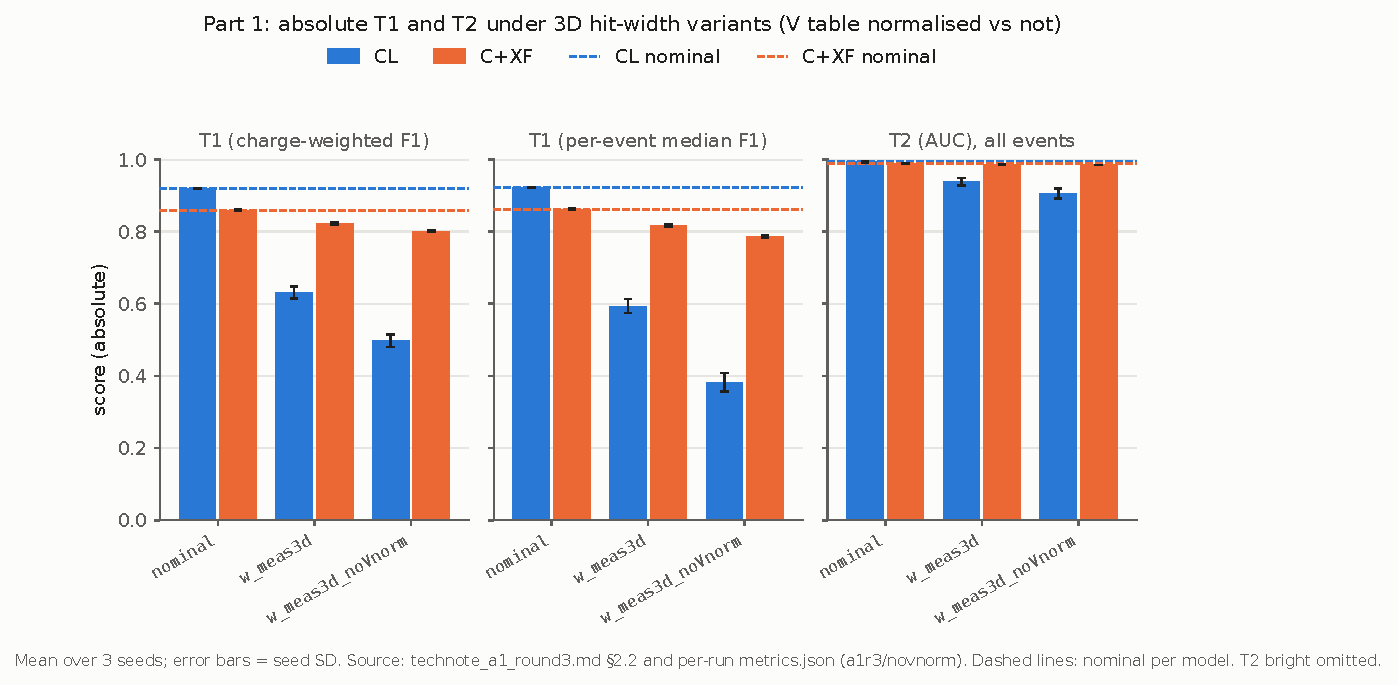
\includegraphics[width=0.92\linewidth,height=0.42\textheight,keepaspectratio]{a1r3_noVnorm_abs.pdf}\caption{Part 1: absolute T1 (charge-weighted and per-event median) and T2 (all events) for nominal, \texttt{w\_\allowbreak{}meas3d} and \texttt{w\_\allowbreak{}meas3d\_\allowbreak{}noVnorm} (§2.2). Dashed lines: nominal per model. T2 bright is not shown. Mean over 3 seeds; error bars = seed SD.}\end{figure}
\begin{figure}[htbp]\centering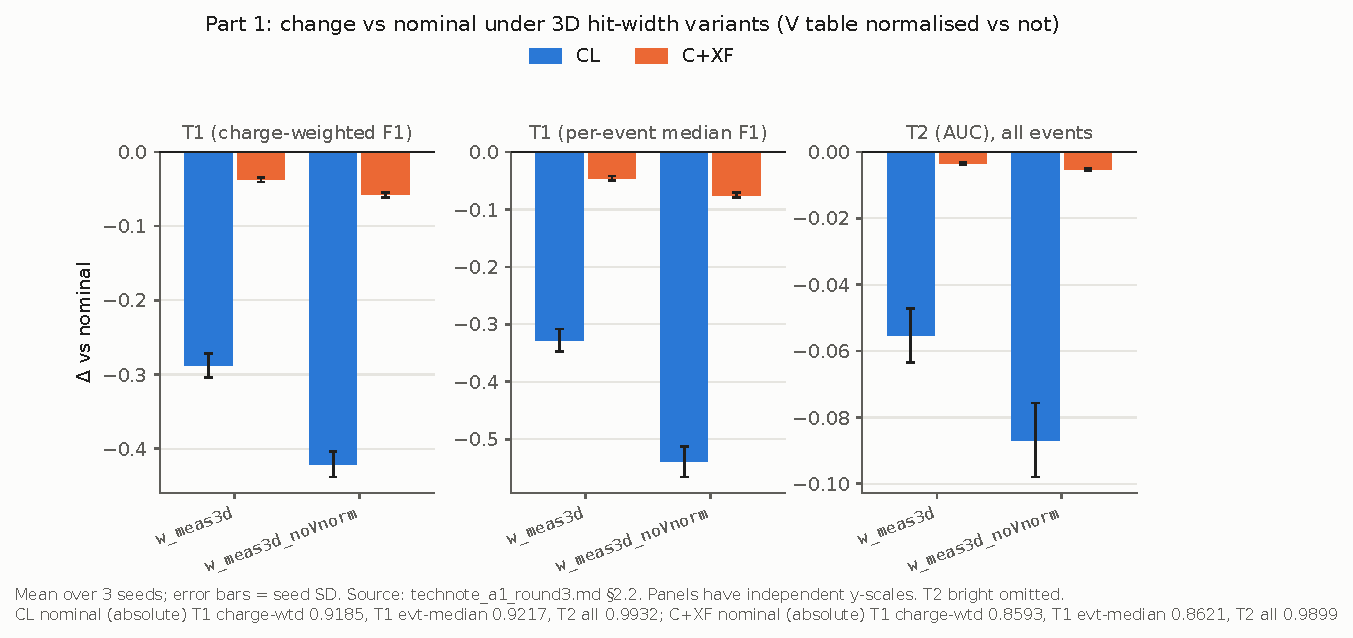
\includegraphics[width=0.92\linewidth,height=0.42\textheight,keepaspectratio]{a1r3_noVnorm_delta.pdf}\caption{Part 1: $\Delta$ T1 and $\Delta$ T2 vs nominal for \texttt{w\_\allowbreak{}meas3d} and \texttt{w\_\allowbreak{}meas3d\_\allowbreak{}noVnorm} (§2.2). T2 bright is not shown. Mean over 3 seeds; error bars = seed SD.}\end{figure}
\subsection{Per-plane T1 charge-weighted ($\Delta$ vs nominal on the plane)}
\textbf{qlfm-M CL}

\begin{center}\footnotesize
\setlength{\tabcolsep}{3pt}\renewcommand{\arraystretch}{1.15}
\begin{tabularx}{\linewidth}{LLLLLL}
\toprule
\textbf{Plane} & \textbf{Nominal} & \textbf{\texttt{w\_\allowbreak{}meas3d}} & \textbf{\texttt{w\_\allowbreak{}meas3d\_\allowbreak{}noVnorm}} & \textbf{\texttt{w\_\allowbreak{}meas3d\_\allowbreak{}V}} & \textbf{\texttt{w\_\allowbreak{}meas3d\_\allowbreak{}noVnorm\_\allowbreak{}V}} \\
\midrule
U & 0.9013 $\pm$ 0.0002 & $-$0.3286 $\pm$ 0.0138 & $-$0.4056 $\pm$ 0.0170 & $-$0.0098 $\pm$ 0.0011 & $-$0.0289 $\pm$ 0.0042 \\
V & 0.9016 $\pm$ 0.0010 & $-$0.2565 $\pm$ 0.0118 & $-$0.5026 $\pm$ 0.0129 & $-$0.0596 $\pm$ 0.0071 & $-$0.3565 $\pm$ 0.0073 \\
Y & 0.9486 $\pm$ 0.0001 & $-$0.2827 $\pm$ 0.0223 & $-$0.3691 $\pm$ 0.0224 & $-$0.0089 $\pm$ 0.0007 & $-$0.0195 $\pm$ 0.0019 \\
\bottomrule
\end{tabularx}
\end{center}
\textbf{qlfm-M C + XF}

\begin{center}\footnotesize
\setlength{\tabcolsep}{3pt}\renewcommand{\arraystretch}{1.15}
\begin{tabularx}{\linewidth}{LLLLLL}
\toprule
\textbf{Plane} & \textbf{Nominal} & \textbf{\texttt{w\_\allowbreak{}meas3d}} & \textbf{\texttt{w\_\allowbreak{}meas3d\_\allowbreak{}noVnorm}} & \textbf{\texttt{w\_\allowbreak{}meas3d\_\allowbreak{}V}} & \textbf{\texttt{w\_\allowbreak{}meas3d\_\allowbreak{}noVnorm\_\allowbreak{}V}} \\
\midrule
U & 0.8392 $\pm$ 0.0024 & $-$0.0471 $\pm$ 0.0056 & $-$0.0447 $\pm$ 0.0051 & +0.0007 $\pm$ 0.0001 & +0.0019 $\pm$ 0.0003 \\
V & 0.8435 $\pm$ 0.0032 & $-$0.0274 $\pm$ 0.0013 & $-$0.0948 $\pm$ 0.0047 & $-$0.0184 $\pm$ 0.0002 & $-$0.0930 $\pm$ 0.0013 \\
Y & 0.8907 $\pm$ 0.0005 & $-$0.0385 $\pm$ 0.0025 & $-$0.0384 $\pm$ 0.0017 & $-$0.0002 $\pm$ 0.0003 & $-$0.0002 $\pm$ 0.0007 \\
\bottomrule
\end{tabularx}
\end{center}
Per-plane per-event-median T1 (paper definition), absolute for \texttt{w\_\allowbreak{}meas3d\_\allowbreak{}noVnorm}, with the round-2 references:

\begin{center}\footnotesize
\setlength{\tabcolsep}{3pt}\renewcommand{\arraystretch}{1.15}
\begin{tabularx}{\linewidth}{LLLLL}
\toprule
\textbf{Model} & \textbf{Plane} & \textbf{\texttt{w\_\allowbreak{}meas3d\_\allowbreak{}noVnorm}} & \textbf{nominal (round 2)} & \textbf{\texttt{w\_\allowbreak{}meas3d} (round 2)} \\
\midrule
CL & U & 0.2757 $\pm$ 0.0123 & 0.8929 $\pm$ 0.0006 & 0.4230 $\pm$ 0.0147 \\
CL & V & 0.1619 $\pm$ 0.0159 & 0.8964 $\pm$ 0.0009 & 0.5990 $\pm$ 0.0138 \\
CL & Y & 0.5187 $\pm$ 0.0433 & 0.9712 $\pm$ 0.0004 & 0.6831 $\pm$ 0.0335 \\
C + XF & U & 0.7495 $\pm$ 0.0065 & 0.8191 $\pm$ 0.0021 & 0.7455 $\pm$ 0.0078 \\
C + XF & V & 0.6784 $\pm$ 0.0046 & 0.8305 $\pm$ 0.0049 & 0.7912 $\pm$ 0.0060 \\
C + XF & Y & 0.8987 $\pm$ 0.0019 & 0.9334 $\pm$ 0.0012 & 0.8977 $\pm$ 0.0023 \\
\bottomrule
\end{tabularx}
\end{center}
\begin{figure}[htbp]\centering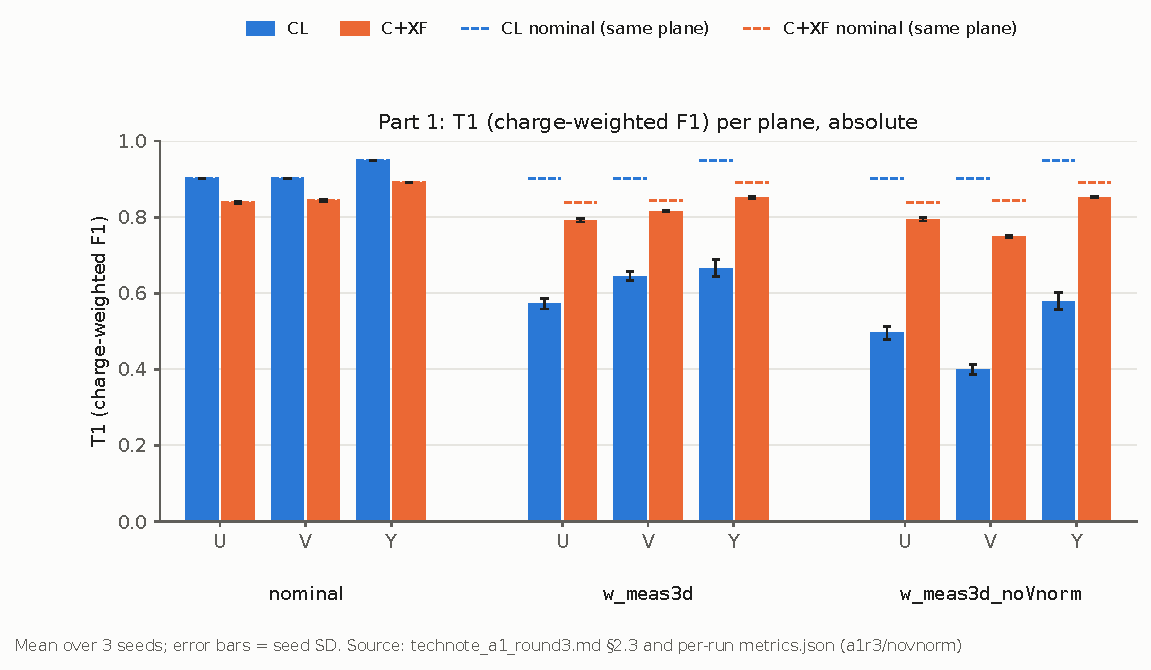
\includegraphics[width=0.92\linewidth,height=0.42\textheight,keepaspectratio]{a1r3_perplane_T1_qwtd_abs.pdf}\caption{Per-plane T1 (charge-weighted), absolute, for nominal, \texttt{w\_\allowbreak{}meas3d} and \texttt{w\_\allowbreak{}meas3d\_\allowbreak{}noVnorm} (§2.3). Dashed segments: same-plane nominal. Mean over 3 seeds; error bars = seed SD.}\end{figure}
\begin{figure}[htbp]\centering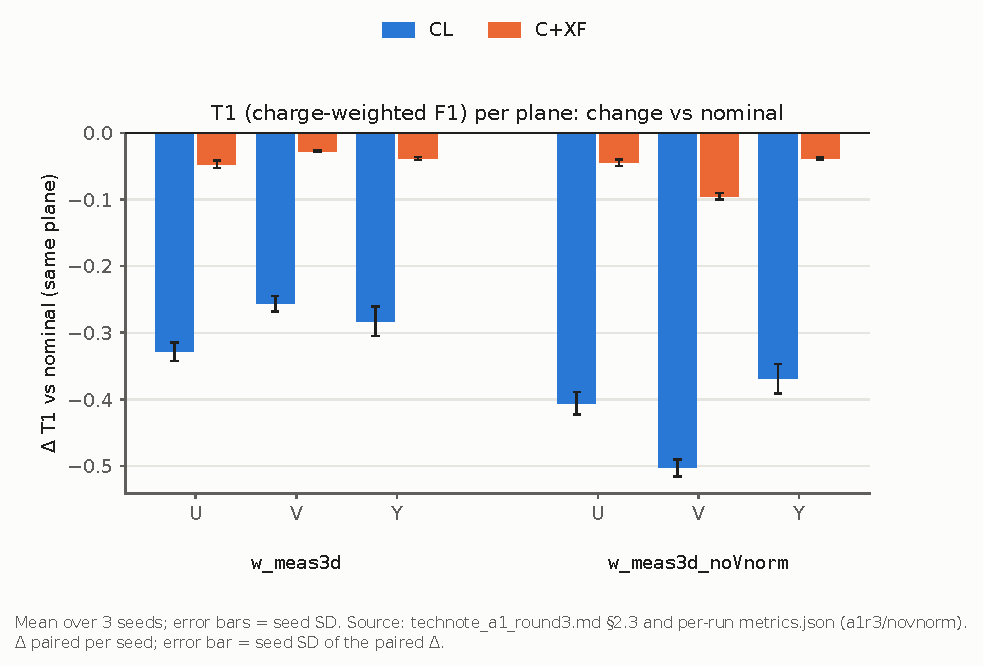
\includegraphics[width=0.92\linewidth,height=0.42\textheight,keepaspectratio]{a1r3_perplane_T1_qwtd_delta.pdf}\caption{Per-plane $\Delta$ T1 (charge-weighted) vs nominal for \texttt{w\_\allowbreak{}meas3d} and \texttt{w\_\allowbreak{}meas3d\_\allowbreak{}noVnorm} (§2.3). $\Delta$ is paired per seed from the per-run \texttt{by\_\allowbreak{}plane} scores; error bars = seed SD of the paired $\Delta$ (mean over 3 seeds).}\end{figure}
\begin{figure}[htbp]\centering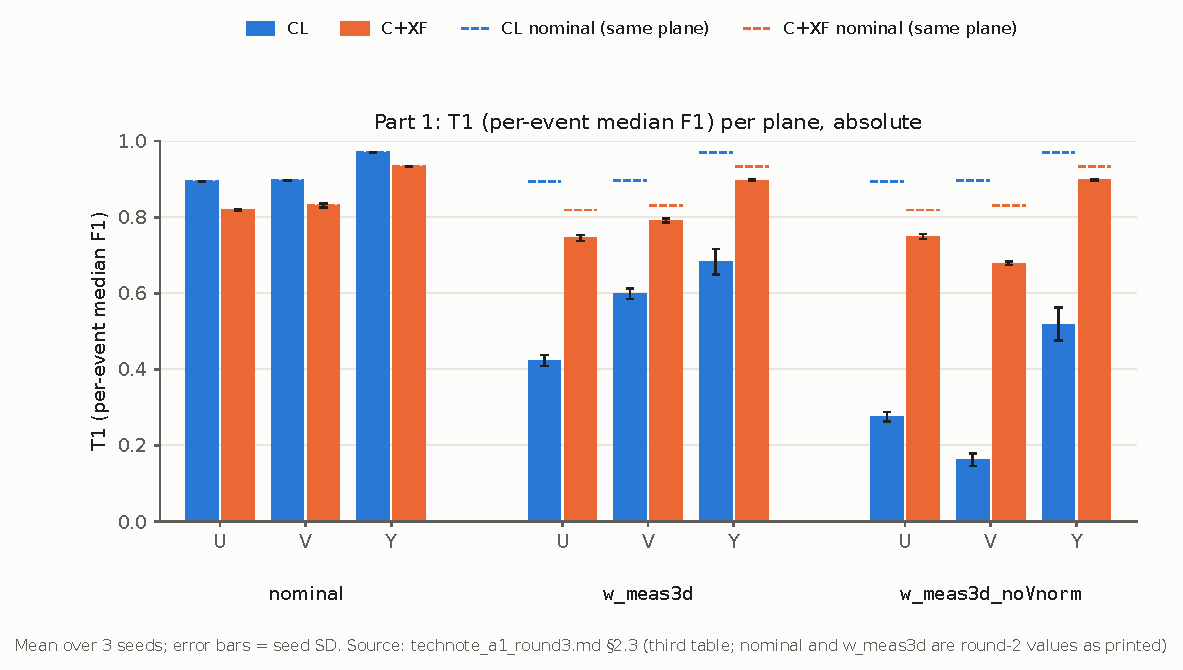
\includegraphics[width=0.92\linewidth,height=0.42\textheight,keepaspectratio]{a1r3_perplane_T1_evtmed_abs.pdf}\caption{Per-plane T1 (per-event median), absolute, for nominal and \texttt{w\_\allowbreak{}meas3d} (round 2) and \texttt{w\_\allowbreak{}meas3d\_\allowbreak{}noVnorm} (§2.3, third table). Dashed segments: same-plane nominal. Mean over 3 seeds; error bars = seed SD as printed in the table.}\end{figure}
\begin{figure}[htbp]\centering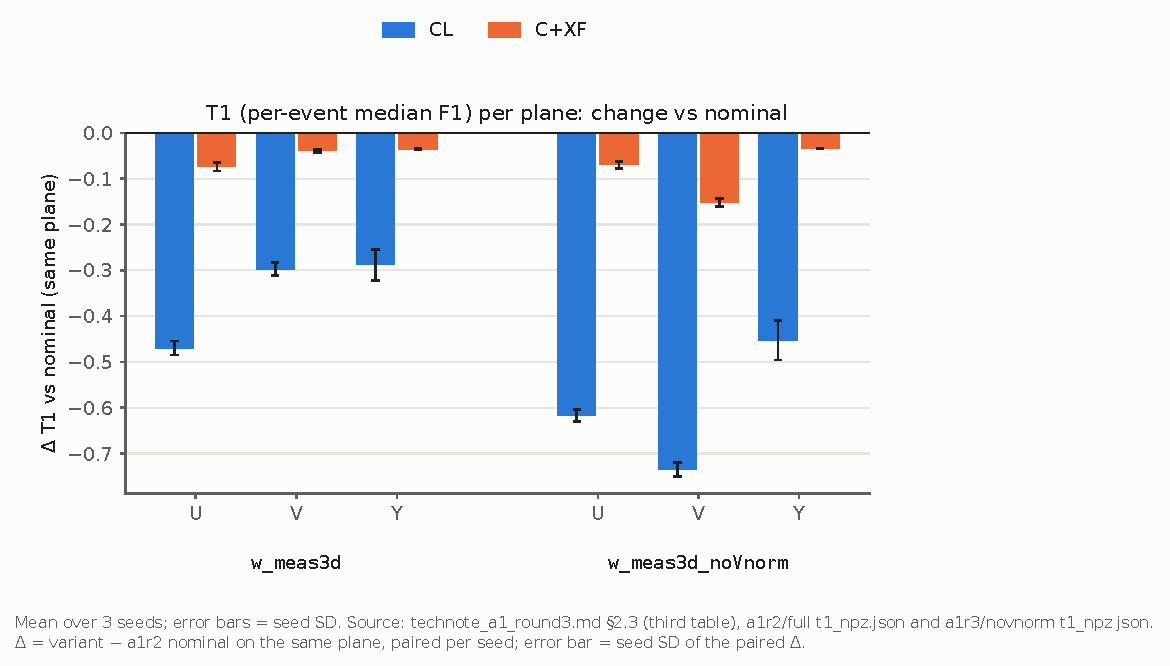
\includegraphics[width=0.92\linewidth,height=0.42\textheight,keepaspectratio]{a1r3_perplane_T1_evtmed_delta.pdf}\caption{Per-plane $\Delta$ T1 (per-event median) vs nominal for \texttt{w\_\allowbreak{}meas3d} (round 2) and \texttt{w\_\allowbreak{}meas3d\_\allowbreak{}noVnorm} (§2.3, third table). $\Delta$ = variant minus the round-2 nominal on the same plane, paired per seed (a1r2 \texttt{t1\_\allowbreak{}npz.json} and the round-3 \texttt{t1\_\allowbreak{}npz} files); error bars = seed SD of the paired $\Delta$ (mean over 3 seeds).}\end{figure}
\subsection{Part 1 findings}
\begin{enumerate}
\item \textbf{The V normalisation is not a detail.} For CL it moves the all-planes T1 loss from $-$0.29 to $-$0.42 (charge-weighted), and the per-event median from $-$0.33 to $-$0.54. For C + XF the loss grows by about half ($-$0.038 $\rightarrow$ $-$0.058).
\item \textbf{In C + XF the extra loss is confined to the V plane.} V drops by $-$0.095 ($-$0.027 normalised), while U and Y match \texttt{w\_\allowbreak{}meas3d} ($-$0.045 and $-$0.038). So its plane contributions remain local, as in round 2.
\item \textbf{In CL the V change spreads to all planes.} All-planes noVnorm costs U $-$0.41, V $-$0.50, Y $-$0.37, against $-$0.33, $-$0.26 and $-$0.28 normalised. V-only noVnorm costs V $-$0.36, but U and Y only $-$0.03 and $-$0.02. As in round 2, CL is more sensitive to interactions between planes than to any one plane.
\item \textbf{Gate 5 passed:} \texttt{w\_\allowbreak{}meas3d} reproduces the round-2 scores in all six models (|$\Delta$T1| $\leq$ 0.0001, |$\Delta$T2| $\leq$ 0.0001).
\end{enumerate}
\section{Part 2: cross-domain pretrain $\rightarrow$ downstream}
\subsection{Domains and runs}
\begin{center}\small
\setlength{\tabcolsep}{3pt}\renewcommand{\arraystretch}{1.15}
\begin{tabularx}{\linewidth}{LL}
\toprule
\textbf{Domain} & \textbf{Definition} \\
\midrule
sim & unaltered open data (\texttt{nominal}) \\
real & \texttt{w\_\allowbreak{}meas3d} widths on simulated-$\nu$ hits and \texttt{l\_\allowbreak{}comb80} on all ophits of flash events (\texttt{d\_\allowbreak{}real}) \\
\bottomrule
\end{tabularx}
\end{center}
The real domain is a modelled data-like domain, not detector data.

\textbf{Event lists.} \texttt{scripts/\allowbreak{}a1r3\_\allowbreak{}make\_\allowbreak{}splits.py} copies the round-1/2 splits and adds \texttt{pre\_\allowbreak{}r3 = pre\_\allowbreak{}f0.90 $-$ (lab\_\allowbreak{}f0.01 $\cup$ val $\cup$ test)}. Pretrain (739 597 events), downstream train (7 471), validation (2 000 per task) and test (10 000 per task) lists are pairwise disjoint and identical across runs. The disjointness was re-checked on the per-run \texttt{event\_\allowbreak{}lists.npz} files (4 pretrain and 24 downstream runs).

The existing models were pretrained on \texttt{pre\_\allowbreak{}f0.90}, which overlaps the downstream training set. That is why the sim backbones are re-pretrained, and why the existing models appear only as a reference row.

\textbf{Backbones (4 new, seed 0, 34 000 steps, 1 node each).}

\begin{center}\small
\setlength{\tabcolsep}{3pt}\renewcommand{\arraystretch}{1.15}
\begin{tabularx}{\linewidth}{LLL}
\toprule
\textbf{Backbone} & \textbf{Light in encoder} & \textbf{Domain} \\
\midrule
\texttt{pre/\allowbreak{}sim\_\allowbreak{}cl} & yes & sim \\
\texttt{pre/\allowbreak{}real\_\allowbreak{}cl} & yes & real \\
\texttt{pre/\allowbreak{}sim\_\allowbreak{}c} & no & sim \\
\texttt{pre/\allowbreak{}real\_\allowbreak{}c} & no & real (widths only) \\
\bottomrule
\end{tabularx}
\end{center}
\textbf{Downstream (24 runs).} Five tasks, 1\% labels, 6 000 steps, batch 32, \texttt{frozen} or \texttt{finetune}. Per model and mode: sim $\rightarrow$ real and real $\rightarrow$ sim at seeds 0 and 1 (16 arm runs), plus sim $\rightarrow$ sim and real $\rightarrow$ real at seed 0 as in-domain controls (8 runs).

\textbf{Evaluations (32).} The 24 runs plus 8 existing-model baselines (\texttt{finetune} seeds 0--2 and \texttt{frozen} seed 0, for each of CL and C + XF). All use \texttt{--absolute-domain}, so \texttt{nominal} is the sim domain and \texttt{d\_\allowbreak{}real} the real domain, whichever domain the model was trained on. This avoids the double perturbation that the round-2 evaluation would apply to models trained in the real domain (checked in Gate 4).

\textbf{Reading the tables.}

\begin{itemize}
\item Rows are labelled pretrain $\rightarrow$ downstream. ``existing (sim) $\rightarrow$ sim'' is the existing yuhw model, pretrained and trained on unaltered data.
\item The \textbf{primary} result is the real-domain evaluation: T1 (charge-weighted and per-event median) and T2 (all events and bright subset).
\item The sim-domain evaluation and the gap (real $-$ sim, per seed) are secondary.
\item C + XF pretraining sees only the width shift, because its backbone is charge-only. Light enters only in its downstream head.
\item Controls and baselines have fewer seeds. Differences between arms smaller than the round-2 seed SD ($\approx$0.002 in T1 for the existing models) should not be read.
\end{itemize}
\subsection{CL, finetune}
\textbf{Primary: real-domain scores}

\begin{center}\footnotesize
\setlength{\tabcolsep}{3pt}\renewcommand{\arraystretch}{1.15}
\begin{tabularx}{\linewidth}{LLLLLL}
\toprule
\textbf{pretrain $\rightarrow$ downstream} & \textbf{n seeds} & \textbf{T1 charge-wtd} & \textbf{T1 evt-median} & \textbf{T2 all} & \textbf{T2 bright} \\
\midrule
real $\rightarrow$ real & 1 & 0.9175 $\pm$ 0.0000 & 0.9203 $\pm$ 0.0000 & 0.9970 $\pm$ 0.0000 & 0.9934 $\pm$ 0.0000 \\
sim $\rightarrow$ real & 2 & 0.9214 $\pm$ 0.0000 & 0.9241 $\pm$ 0.0001 & 0.9961 $\pm$ 0.0000 & 0.9939 $\pm$ 0.0013 \\
real $\rightarrow$ sim & 2 & 0.6658 $\pm$ 0.0032 & 0.6219 $\pm$ 0.0015 & 0.9658 $\pm$ 0.0073 & 0.9583 $\pm$ 0.0016 \\
sim $\rightarrow$ sim & 1 & 0.5981 $\pm$ 0.0000 & 0.5213 $\pm$ 0.0000 & 0.9293 $\pm$ 0.0000 & 0.9002 $\pm$ 0.0000 \\
existing (sim) $\rightarrow$ sim & 3 & 0.6210 $\pm$ 0.0128 & 0.5709 $\pm$ 0.0165 & 0.9400 $\pm$ 0.0116 & 0.9135 $\pm$ 0.0222 \\
\bottomrule
\end{tabularx}
\end{center}
\textbf{Secondary: sim-domain scores and domain gap}

\begin{center}\scriptsize
\setlength{\tabcolsep}{3pt}\renewcommand{\arraystretch}{1.15}
\begin{tabularx}{\linewidth}{LLLLLLLLL}
\toprule
\textbf{pretrain $\rightarrow$ downstream} & \textbf{T1 cw (sim)} & \textbf{T1 med (sim)} & \textbf{T2 all (sim)} & \textbf{T2 bright (sim)} & \textbf{gap T1 cw} & \textbf{gap T1 med} & \textbf{gap T2 all} & \textbf{gap T2 bright} \\
\midrule
real $\rightarrow$ real & 0.6827 $\pm$ 0.0000 & 0.6748 $\pm$ 0.0000 & 0.9651 $\pm$ 0.0000 & 0.9482 $\pm$ 0.0000 & +0.2348 $\pm$ 0.0000 & +0.2455 $\pm$ 0.0000 & +0.0318 $\pm$ 0.0000 & +0.0451 $\pm$ 0.0000 \\
sim $\rightarrow$ real & 0.7151 $\pm$ 0.0153 & 0.7352 $\pm$ 0.0240 & 0.9651 $\pm$ 0.0091 & 0.9566 $\pm$ 0.0041 & +0.2063 $\pm$ 0.0154 & +0.1890 $\pm$ 0.0241 & +0.0310 $\pm$ 0.0092 & +0.0374 $\pm$ 0.0054 \\
real $\rightarrow$ sim & 0.9220 $\pm$ 0.0013 & 0.9265 $\pm$ 0.0023 & 0.9976 $\pm$ 0.0004 & 0.9956 $\pm$ 0.0006 & -0.2562 $\pm$ 0.0045 & -0.3046 $\pm$ 0.0008 & -0.0318 $\pm$ 0.0077 & -0.0374 $\pm$ 0.0023 \\
sim $\rightarrow$ sim & 0.9252 $\pm$ 0.0000 & 0.9290 $\pm$ 0.0000 & 0.9947 $\pm$ 0.0000 & 0.9911 $\pm$ 0.0000 & -0.3270 $\pm$ 0.0000 & -0.4077 $\pm$ 0.0000 & -0.0654 $\pm$ 0.0000 & -0.0909 $\pm$ 0.0000 \\
existing (sim) $\rightarrow$ sim & 0.9185 $\pm$ 0.0002 & 0.9217 $\pm$ 0.0006 & 0.9932 $\pm$ 0.0028 & 0.9882 $\pm$ 0.0035 & -0.2975 $\pm$ 0.0128 & -0.3508 $\pm$ 0.0170 & -0.0532 $\pm$ 0.0087 & -0.0746 $\pm$ 0.0193 \\
\bottomrule
\end{tabularx}
\end{center}
\textbf{Decomposition of the real-domain change in T1 charge-weighted ($\Delta$ vs the sim-domain score of the same run)}

\begin{center}\footnotesize
\setlength{\tabcolsep}{3pt}\renewcommand{\arraystretch}{1.15}
\begin{tabularx}{\linewidth}{LLLLL}
\toprule
\textbf{pretrain $\rightarrow$ downstream} & \textbf{width only (\texttt{w\_\allowbreak{}meas3d})} & \textbf{light only (\texttt{l\_\allowbreak{}comb80})} & \textbf{\texttt{d\_\allowbreak{}real}} & \textbf{\texttt{d\_\allowbreak{}real\_\allowbreak{}noVnorm} (absolute T1 cw)} \\
\midrule
real $\rightarrow$ real & +0.2346 $\pm$ 0.0000 & -0.0052 $\pm$ 0.0000 & +0.2348 $\pm$ 0.0000 & 0.8102 $\pm$ 0.0000 \\
sim $\rightarrow$ real & +0.2062 $\pm$ 0.0157 & -0.0019 $\pm$ 0.0011 & +0.2063 $\pm$ 0.0154 & 0.8274 $\pm$ 0.0023 \\
real $\rightarrow$ sim & -0.2421 $\pm$ 0.0005 & -0.0010 $\pm$ 0.0004 & -0.2562 $\pm$ 0.0045 & 0.5157 $\pm$ 0.0103 \\
sim $\rightarrow$ sim & -0.3210 $\pm$ 0.0000 & -0.0007 $\pm$ 0.0000 & -0.3270 $\pm$ 0.0000 & 0.4681 $\pm$ 0.0000 \\
existing (sim) $\rightarrow$ sim & -0.2877 $\pm$ 0.0164 & -0.0010 $\pm$ 0.0002 & -0.2975 $\pm$ 0.0128 & 0.4861 $\pm$ 0.0116 \\
\bottomrule
\end{tabularx}
\end{center}
\textbf{Per-plane T1 per-event median, real domain}

\begin{center}\small
\setlength{\tabcolsep}{3pt}\renewcommand{\arraystretch}{1.15}
\begin{tabularx}{\linewidth}{LLLL}
\toprule
\textbf{pretrain $\rightarrow$ downstream} & \textbf{U} & \textbf{V} & \textbf{Y} \\
\midrule
real $\rightarrow$ real & 0.9010 $\pm$ 0.0000 & 0.8952 $\pm$ 0.0000 & 0.9695 $\pm$ 0.0000 \\
sim $\rightarrow$ real & 0.9033 $\pm$ 0.0001 & 0.9043 $\pm$ 0.0019 & 0.9734 $\pm$ 0.0001 \\
real $\rightarrow$ sim & 0.4104 $\pm$ 0.0051 & 0.6765 $\pm$ 0.0075 & 0.7028 $\pm$ 0.0123 \\
sim $\rightarrow$ sim & 0.2671 $\pm$ 0.0000 & 0.6198 $\pm$ 0.0000 & 0.5660 $\pm$ 0.0000 \\
existing (sim) $\rightarrow$ sim & 0.3914 $\pm$ 0.0099 & 0.5698 $\pm$ 0.0117 & 0.6585 $\pm$ 0.0288 \\
\bottomrule
\end{tabularx}
\end{center}
\subsection{CL, frozen}
\textbf{Primary: real-domain scores}

\begin{center}\footnotesize
\setlength{\tabcolsep}{3pt}\renewcommand{\arraystretch}{1.15}
\begin{tabularx}{\linewidth}{LLLLLL}
\toprule
\textbf{pretrain $\rightarrow$ downstream} & \textbf{n seeds} & \textbf{T1 charge-wtd} & \textbf{T1 evt-median} & \textbf{T2 all} & \textbf{T2 bright} \\
\midrule
real $\rightarrow$ real & 1 & 0.8934 $\pm$ 0.0000 & 0.8920 $\pm$ 0.0000 & 0.9964 $\pm$ 0.0000 & 0.9882 $\pm$ 0.0000 \\
sim $\rightarrow$ real & 2 & 0.8448 $\pm$ 0.0008 & 0.8340 $\pm$ 0.0014 & 0.9886 $\pm$ 0.0008 & 0.9603 $\pm$ 0.0039 \\
real $\rightarrow$ sim & 2 & 0.7626 $\pm$ 0.0045 & 0.7175 $\pm$ 0.0053 & 0.9928 $\pm$ 0.0009 & 0.9709 $\pm$ 0.0040 \\
sim $\rightarrow$ sim & 1 & 0.4958 $\pm$ 0.0000 & 0.2434 $\pm$ 0.0000 & 0.9818 $\pm$ 0.0000 & 0.9471 $\pm$ 0.0000 \\
existing (sim) $\rightarrow$ sim & 1 & 0.4736 $\pm$ 0.0000 & 0.2431 $\pm$ 0.0000 & 0.9770 $\pm$ 0.0000 & 0.9363 $\pm$ 0.0000 \\
\bottomrule
\end{tabularx}
\end{center}
\textbf{Secondary: sim-domain scores and domain gap}

\begin{center}\scriptsize
\setlength{\tabcolsep}{3pt}\renewcommand{\arraystretch}{1.15}
\begin{tabularx}{\linewidth}{LLLLLLLLL}
\toprule
\textbf{pretrain $\rightarrow$ downstream} & \textbf{T1 cw (sim)} & \textbf{T1 med (sim)} & \textbf{T2 all (sim)} & \textbf{T2 bright (sim)} & \textbf{gap T1 cw} & \textbf{gap T1 med} & \textbf{gap T2 all} & \textbf{gap T2 bright} \\
\midrule
real $\rightarrow$ real & 0.5175 $\pm$ 0.0000 & 0.3878 $\pm$ 0.0000 & 0.9785 $\pm$ 0.0000 & 0.9322 $\pm$ 0.0000 & +0.3759 $\pm$ 0.0000 & +0.5042 $\pm$ 0.0000 & +0.0180 $\pm$ 0.0000 & +0.0559 $\pm$ 0.0000 \\
sim $\rightarrow$ real & 0.7669 $\pm$ 0.0072 & 0.7314 $\pm$ 0.0109 & 0.9867 $\pm$ 0.0007 & 0.9514 $\pm$ 0.0039 & +0.0779 $\pm$ 0.0064 & +0.1026 $\pm$ 0.0096 & +0.0019 $\pm$ 0.0001 & +0.0088 $\pm$ 0.0001 \\
real $\rightarrow$ sim & 0.8681 $\pm$ 0.0005 & 0.8681 $\pm$ 0.0001 & 0.9880 $\pm$ 0.0010 & 0.9553 $\pm$ 0.0042 & -0.1055 $\pm$ 0.0041 & -0.1506 $\pm$ 0.0053 & +0.0048 $\pm$ 0.0000 & +0.0155 $\pm$ 0.0002 \\
sim $\rightarrow$ sim & 0.8932 $\pm$ 0.0000 & 0.8936 $\pm$ 0.0000 & 0.9963 $\pm$ 0.0000 & 0.9855 $\pm$ 0.0000 & -0.3974 $\pm$ 0.0000 & -0.6502 $\pm$ 0.0000 & -0.0145 $\pm$ 0.0000 & -0.0385 $\pm$ 0.0000 \\
existing (sim) $\rightarrow$ sim & 0.8944 $\pm$ 0.0000 & 0.8939 $\pm$ 0.0000 & 0.9971 $\pm$ 0.0000 & 0.9892 $\pm$ 0.0000 & -0.4208 $\pm$ 0.0000 & -0.6508 $\pm$ 0.0000 & -0.0201 $\pm$ 0.0000 & -0.0529 $\pm$ 0.0000 \\
\bottomrule
\end{tabularx}
\end{center}
\textbf{Decomposition}

\begin{center}\footnotesize
\setlength{\tabcolsep}{3pt}\renewcommand{\arraystretch}{1.15}
\begin{tabularx}{\linewidth}{LLLLL}
\toprule
\textbf{pretrain $\rightarrow$ downstream} & \textbf{width only (\texttt{w\_\allowbreak{}meas3d})} & \textbf{light only (\texttt{l\_\allowbreak{}comb80})} & \textbf{\texttt{d\_\allowbreak{}real}} & \textbf{\texttt{d\_\allowbreak{}real\_\allowbreak{}noVnorm} (absolute T1 cw)} \\
\midrule
real $\rightarrow$ real & +0.3755 $\pm$ 0.0000 & +0.0058 $\pm$ 0.0000 & +0.3759 $\pm$ 0.0000 & 0.7291 $\pm$ 0.0000 \\
sim $\rightarrow$ real & +0.0785 $\pm$ 0.0066 & -0.0039 $\pm$ 0.0009 & +0.0779 $\pm$ 0.0064 & 0.7178 $\pm$ 0.0011 \\
real $\rightarrow$ sim & -0.0985 $\pm$ 0.0039 & -0.0013 $\pm$ 0.0001 & -0.1055 $\pm$ 0.0041 & 0.5525 $\pm$ 0.0026 \\
sim $\rightarrow$ sim & -0.3918 $\pm$ 0.0000 & -0.0000 $\pm$ 0.0000 & -0.3974 $\pm$ 0.0000 & 0.3441 $\pm$ 0.0000 \\
existing (sim) $\rightarrow$ sim & -0.4117 $\pm$ 0.0000 & -0.0005 $\pm$ 0.0000 & -0.4208 $\pm$ 0.0000 & 0.2782 $\pm$ 0.0000 \\
\bottomrule
\end{tabularx}
\end{center}
\textbf{Per-plane T1 per-event median, real domain}

\begin{center}\small
\setlength{\tabcolsep}{3pt}\renewcommand{\arraystretch}{1.15}
\begin{tabularx}{\linewidth}{LLLL}
\toprule
\textbf{pretrain $\rightarrow$ downstream} & \textbf{U} & \textbf{V} & \textbf{Y} \\
\midrule
real $\rightarrow$ real & 0.8624 $\pm$ 0.0000 & 0.8454 $\pm$ 0.0000 & 0.9590 $\pm$ 0.0000 \\
sim $\rightarrow$ real & 0.7610 $\pm$ 0.0013 & 0.7882 $\pm$ 0.0002 & 0.9342 $\pm$ 0.0005 \\
real $\rightarrow$ sim & 0.6780 $\pm$ 0.0107 & 0.6958 $\pm$ 0.0012 & 0.8007 $\pm$ 0.0041 \\
sim $\rightarrow$ sim & 0.0664 $\pm$ 0.0000 & 0.3003 $\pm$ 0.0000 & 0.2053 $\pm$ 0.0000 \\
existing (sim) $\rightarrow$ sim & 0.1008 $\pm$ 0.0000 & 0.2341 $\pm$ 0.0000 & 0.2456 $\pm$ 0.0000 \\
\bottomrule
\end{tabularx}
\end{center}
\subsection{C + XF, finetune}
\textbf{Primary: real-domain scores}

\begin{center}\footnotesize
\setlength{\tabcolsep}{3pt}\renewcommand{\arraystretch}{1.15}
\begin{tabularx}{\linewidth}{LLLLLL}
\toprule
\textbf{pretrain $\rightarrow$ downstream} & \textbf{n seeds} & \textbf{T1 charge-wtd} & \textbf{T1 evt-median} & \textbf{T2 all} & \textbf{T2 bright} \\
\midrule
real $\rightarrow$ real & 1 & 0.8813 $\pm$ 0.0000 & 0.8880 $\pm$ 0.0000 & 0.9833 $\pm$ 0.0000 & 0.9633 $\pm$ 0.0000 \\
sim $\rightarrow$ real & 2 & 0.8294 $\pm$ 0.0064 & 0.8223 $\pm$ 0.0096 & 0.9856 $\pm$ 0.0012 & 0.9568 $\pm$ 0.0051 \\
real $\rightarrow$ sim & 2 & 0.8076 $\pm$ 0.0077 & 0.7980 $\pm$ 0.0155 & 0.9803 $\pm$ 0.0008 & 0.9521 $\pm$ 0.0022 \\
sim $\rightarrow$ sim & 1 & 0.7667 $\pm$ 0.0000 & 0.7298 $\pm$ 0.0000 & 0.9847 $\pm$ 0.0000 & 0.9565 $\pm$ 0.0000 \\
existing (sim) $\rightarrow$ sim & 3 & 0.8084 $\pm$ 0.0019 & 0.7901 $\pm$ 0.0028 & 0.9865 $\pm$ 0.0005 & 0.9604 $\pm$ 0.0009 \\
\bottomrule
\end{tabularx}
\end{center}
\textbf{Secondary: sim-domain scores and domain gap}

\begin{center}\scriptsize
\setlength{\tabcolsep}{3pt}\renewcommand{\arraystretch}{1.15}
\begin{tabularx}{\linewidth}{LLLLLLLLL}
\toprule
\textbf{pretrain $\rightarrow$ downstream} & \textbf{T1 cw (sim)} & \textbf{T1 med (sim)} & \textbf{T2 all (sim)} & \textbf{T2 bright (sim)} & \textbf{gap T1 cw} & \textbf{gap T1 med} & \textbf{gap T2 all} & \textbf{gap T2 bright} \\
\midrule
real $\rightarrow$ real & 0.8603 $\pm$ 0.0000 & 0.8698 $\pm$ 0.0000 & 0.9744 $\pm$ 0.0000 & 0.9509 $\pm$ 0.0000 & +0.0210 $\pm$ 0.0000 & +0.0182 $\pm$ 0.0000 & +0.0090 $\pm$ 0.0000 & +0.0125 $\pm$ 0.0000 \\
sim $\rightarrow$ real & 0.8223 $\pm$ 0.0055 & 0.8238 $\pm$ 0.0069 & 0.9817 $\pm$ 0.0012 & 0.9470 $\pm$ 0.0052 & +0.0071 $\pm$ 0.0009 & -0.0015 $\pm$ 0.0027 & +0.0039 $\pm$ 0.0000 & +0.0097 $\pm$ 0.0001 \\
real $\rightarrow$ sim & 0.8999 $\pm$ 0.0001 & 0.9097 $\pm$ 0.0003 & 0.9905 $\pm$ 0.0008 & 0.9742 $\pm$ 0.0018 & -0.0923 $\pm$ 0.0078 & -0.1116 $\pm$ 0.0152 & -0.0102 $\pm$ 0.0000 & -0.0221 $\pm$ 0.0005 \\
sim $\rightarrow$ sim & 0.8654 $\pm$ 0.0000 & 0.8678 $\pm$ 0.0000 & 0.9921 $\pm$ 0.0000 & 0.9743 $\pm$ 0.0000 & -0.0987 $\pm$ 0.0000 & -0.1380 $\pm$ 0.0000 & -0.0074 $\pm$ 0.0000 & -0.0178 $\pm$ 0.0000 \\
existing (sim) $\rightarrow$ sim & 0.8593 $\pm$ 0.0017 & 0.8623 $\pm$ 0.0014 & 0.9899 $\pm$ 0.0005 & 0.9689 $\pm$ 0.0004 & -0.0509 $\pm$ 0.0022 & -0.0722 $\pm$ 0.0024 & -0.0034 $\pm$ 0.0005 & -0.0084 $\pm$ 0.0011 \\
\bottomrule
\end{tabularx}
\end{center}
\textbf{Decomposition}

\begin{center}\footnotesize
\setlength{\tabcolsep}{3pt}\renewcommand{\arraystretch}{1.15}
\begin{tabularx}{\linewidth}{LLLLL}
\toprule
\textbf{pretrain $\rightarrow$ downstream} & \textbf{width only (\texttt{w\_\allowbreak{}meas3d})} & \textbf{light only (\texttt{l\_\allowbreak{}comb80})} & \textbf{\texttt{d\_\allowbreak{}real}} & \textbf{\texttt{d\_\allowbreak{}real\_\allowbreak{}noVnorm} (absolute T1 cw)} \\
\midrule
real $\rightarrow$ real & +0.0181 $\pm$ 0.0000 & -0.0001 $\pm$ 0.0000 & +0.0210 $\pm$ 0.0000 & 0.8608 $\pm$ 0.0000 \\
sim $\rightarrow$ real & +0.0025 $\pm$ 0.0005 & +0.0035 $\pm$ 0.0004 & +0.0071 $\pm$ 0.0009 & 0.8235 $\pm$ 0.0082 \\
real $\rightarrow$ sim & -0.0816 $\pm$ 0.0038 & -0.0044 $\pm$ 0.0010 & -0.0923 $\pm$ 0.0078 & 0.7477 $\pm$ 0.0097 \\
sim $\rightarrow$ sim & -0.0817 $\pm$ 0.0000 & -0.0094 $\pm$ 0.0000 & -0.0987 $\pm$ 0.0000 & 0.7116 $\pm$ 0.0000 \\
existing (sim) $\rightarrow$ sim & -0.0375 $\pm$ 0.0030 & -0.0099 $\pm$ 0.0003 & -0.0509 $\pm$ 0.0022 & 0.7875 $\pm$ 0.0013 \\
\bottomrule
\end{tabularx}
\end{center}
\textbf{Per-plane T1 per-event median, real domain}

\begin{center}\small
\setlength{\tabcolsep}{3pt}\renewcommand{\arraystretch}{1.15}
\begin{tabularx}{\linewidth}{LLLL}
\toprule
\textbf{pretrain $\rightarrow$ downstream} & \textbf{U} & \textbf{V} & \textbf{Y} \\
\midrule
real $\rightarrow$ real & 0.8561 $\pm$ 0.0000 & 0.8631 $\pm$ 0.0000 & 0.9479 $\pm$ 0.0000 \\
sim $\rightarrow$ real & 0.7732 $\pm$ 0.0166 & 0.7845 $\pm$ 0.0109 & 0.9091 $\pm$ 0.0056 \\
real $\rightarrow$ sim & 0.7102 $\pm$ 0.0155 & 0.8220 $\pm$ 0.0030 & 0.8710 $\pm$ 0.0158 \\
sim $\rightarrow$ sim & 0.6061 $\pm$ 0.0000 & 0.7259 $\pm$ 0.0000 & 0.8292 $\pm$ 0.0000 \\
existing (sim) $\rightarrow$ sim & 0.7146 $\pm$ 0.0055 & 0.7638 $\pm$ 0.0040 & 0.8742 $\pm$ 0.0020 \\
\bottomrule
\end{tabularx}
\end{center}
\begin{figure}[htbp]\centering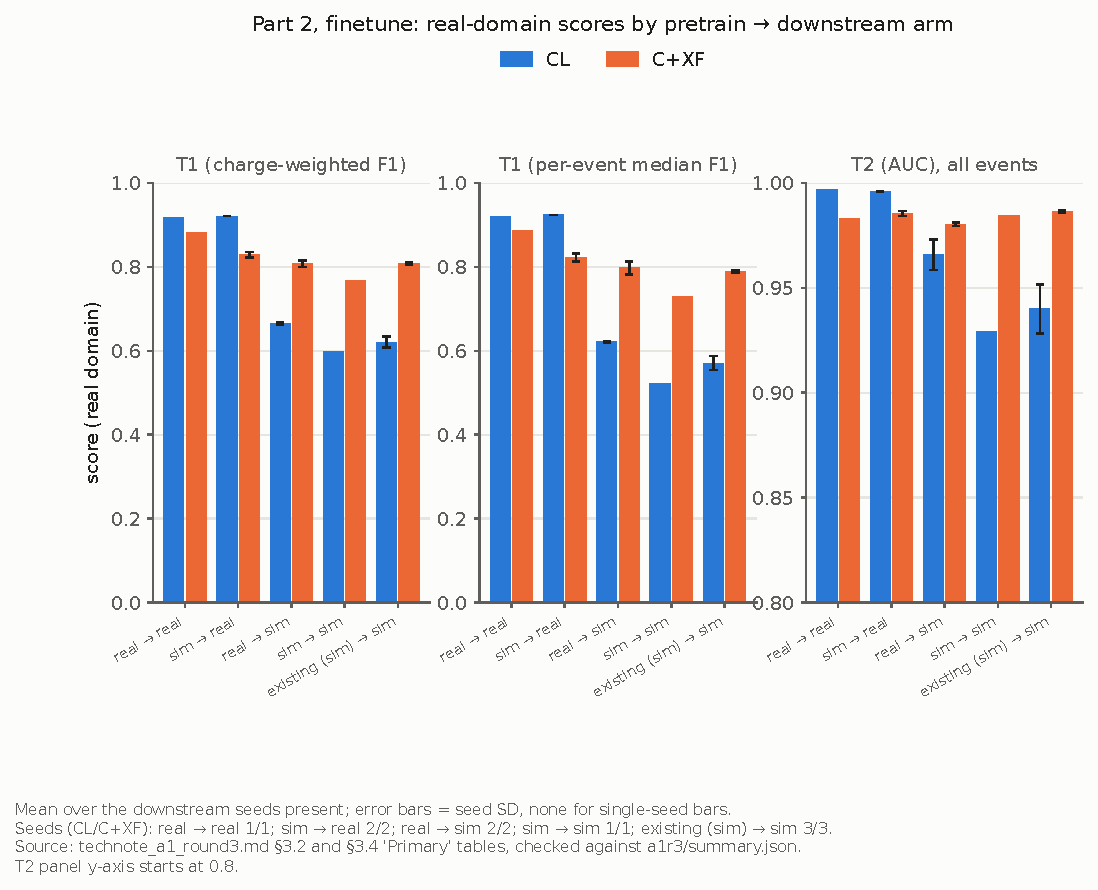
\includegraphics[width=0.92\linewidth,height=0.42\textheight,keepaspectratio]{a1r3_part2_finetune_primary.pdf}\caption{Part 2, finetune: real-domain T1 (charge-weighted and per-event median) and T2 (all events) by pretrain $\rightarrow$ downstream arm, for CL (§3.2) and C + XF (§3.4), 'Primary' tables. Mean $\pm$ seed SD over the seeds present; single-seed arms have no error bar.}\end{figure}
\subsection{C + XF, frozen}
\textbf{Primary: real-domain scores}

\begin{center}\footnotesize
\setlength{\tabcolsep}{3pt}\renewcommand{\arraystretch}{1.15}
\begin{tabularx}{\linewidth}{LLLLLL}
\toprule
\textbf{pretrain $\rightarrow$ downstream} & \textbf{n seeds} & \textbf{T1 charge-wtd} & \textbf{T1 evt-median} & \textbf{T2 all} & \textbf{T2 bright} \\
\midrule
real $\rightarrow$ real & 1 & 0.7413 $\pm$ 0.0000 & 0.6903 $\pm$ 0.0000 & 0.9845 $\pm$ 0.0000 & 0.9484 $\pm$ 0.0000 \\
sim $\rightarrow$ real & 2 & 0.6835 $\pm$ 0.0006 & 0.6100 $\pm$ 0.0003 & 0.9821 $\pm$ 0.0009 & 0.9340 $\pm$ 0.0027 \\
real $\rightarrow$ sim & 2 & 0.6983 $\pm$ 0.0076 & 0.6217 $\pm$ 0.0150 & 0.9840 $\pm$ 0.0020 & 0.9517 $\pm$ 0.0016 \\
sim $\rightarrow$ sim & 1 & 0.6385 $\pm$ 0.0000 & 0.5361 $\pm$ 0.0000 & 0.9814 $\pm$ 0.0000 & 0.9367 $\pm$ 0.0000 \\
existing (sim) $\rightarrow$ sim & 1 & 0.6486 $\pm$ 0.0000 & 0.5506 $\pm$ 0.0000 & 0.9843 $\pm$ 0.0000 & 0.9461 $\pm$ 0.0000 \\
\bottomrule
\end{tabularx}
\end{center}
\textbf{Secondary: sim-domain scores and domain gap}

\begin{center}\scriptsize
\setlength{\tabcolsep}{3pt}\renewcommand{\arraystretch}{1.15}
\begin{tabularx}{\linewidth}{LLLLLLLLL}
\toprule
\textbf{pretrain $\rightarrow$ downstream} & \textbf{T1 cw (sim)} & \textbf{T1 med (sim)} & \textbf{T2 all (sim)} & \textbf{T2 bright (sim)} & \textbf{gap T1 cw} & \textbf{gap T1 med} & \textbf{gap T2 all} & \textbf{gap T2 bright} \\
\midrule
real $\rightarrow$ real & 0.7393 $\pm$ 0.0000 & 0.6989 $\pm$ 0.0000 & 0.9805 $\pm$ 0.0000 & 0.9388 $\pm$ 0.0000 & +0.0020 $\pm$ 0.0000 & -0.0086 $\pm$ 0.0000 & +0.0040 $\pm$ 0.0000 & +0.0096 $\pm$ 0.0000 \\
sim $\rightarrow$ real & 0.6857 $\pm$ 0.0019 & 0.6226 $\pm$ 0.0088 & 0.9783 $\pm$ 0.0016 & 0.9211 $\pm$ 0.0050 & -0.0022 $\pm$ 0.0025 & -0.0125 $\pm$ 0.0092 & +0.0038 $\pm$ 0.0007 & +0.0129 $\pm$ 0.0023 \\
real $\rightarrow$ sim & 0.7604 $\pm$ 0.0021 & 0.7297 $\pm$ 0.0070 & 0.9860 $\pm$ 0.0010 & 0.9513 $\pm$ 0.0009 & -0.0621 $\pm$ 0.0056 & -0.1080 $\pm$ 0.0080 & -0.0019 $\pm$ 0.0010 & +0.0003 $\pm$ 0.0025 \\
sim $\rightarrow$ sim & 0.7136 $\pm$ 0.0000 & 0.6630 $\pm$ 0.0000 & 0.9811 $\pm$ 0.0000 & 0.9319 $\pm$ 0.0000 & -0.0751 $\pm$ 0.0000 & -0.1269 $\pm$ 0.0000 & +0.0003 $\pm$ 0.0000 & +0.0049 $\pm$ 0.0000 \\
existing (sim) $\rightarrow$ sim & 0.7207 $\pm$ 0.0000 & 0.6627 $\pm$ 0.0000 & 0.9839 $\pm$ 0.0000 & 0.9433 $\pm$ 0.0000 & -0.0722 $\pm$ 0.0000 & -0.1120 $\pm$ 0.0000 & +0.0004 $\pm$ 0.0000 & +0.0028 $\pm$ 0.0000 \\
\bottomrule
\end{tabularx}
\end{center}
\textbf{Decomposition}

\begin{center}\footnotesize
\setlength{\tabcolsep}{3pt}\renewcommand{\arraystretch}{1.15}
\begin{tabularx}{\linewidth}{LLLLL}
\toprule
\textbf{pretrain $\rightarrow$ downstream} & \textbf{width only (\texttt{w\_\allowbreak{}meas3d})} & \textbf{light only (\texttt{l\_\allowbreak{}comb80})} & \textbf{\texttt{d\_\allowbreak{}real}} & \textbf{\texttt{d\_\allowbreak{}real\_\allowbreak{}noVnorm} (absolute T1 cw)} \\
\midrule
real $\rightarrow$ real & -0.0024 $\pm$ 0.0000 & +0.0039 $\pm$ 0.0000 & +0.0020 $\pm$ 0.0000 & 0.7329 $\pm$ 0.0000 \\
sim $\rightarrow$ real & -0.0058 $\pm$ 0.0003 & +0.0031 $\pm$ 0.0020 & -0.0022 $\pm$ 0.0025 & 0.6814 $\pm$ 0.0022 \\
real $\rightarrow$ sim & -0.0419 $\pm$ 0.0009 & -0.0148 $\pm$ 0.0047 & -0.0621 $\pm$ 0.0056 & 0.6724 $\pm$ 0.0071 \\
sim $\rightarrow$ sim & -0.0502 $\pm$ 0.0000 & -0.0219 $\pm$ 0.0000 & -0.0751 $\pm$ 0.0000 & 0.6147 $\pm$ 0.0000 \\
existing (sim) $\rightarrow$ sim & -0.0466 $\pm$ 0.0000 & -0.0218 $\pm$ 0.0000 & -0.0722 $\pm$ 0.0000 & 0.6254 $\pm$ 0.0000 \\
\bottomrule
\end{tabularx}
\end{center}
\textbf{Per-plane T1 per-event median, real domain}

\begin{center}\small
\setlength{\tabcolsep}{3pt}\renewcommand{\arraystretch}{1.15}
\begin{tabularx}{\linewidth}{LLLL}
\toprule
\textbf{pretrain $\rightarrow$ downstream} & \textbf{U} & \textbf{V} & \textbf{Y} \\
\midrule
real $\rightarrow$ real & 0.5949 $\pm$ 0.0000 & 0.6199 $\pm$ 0.0000 & 0.8152 $\pm$ 0.0000 \\
sim $\rightarrow$ real & 0.4650 $\pm$ 0.0004 & 0.4775 $\pm$ 0.0104 & 0.7702 $\pm$ 0.0040 \\
real $\rightarrow$ sim & 0.4885 $\pm$ 0.0147 & 0.5682 $\pm$ 0.0153 & 0.7417 $\pm$ 0.0164 \\
sim $\rightarrow$ sim & 0.3506 $\pm$ 0.0000 & 0.4320 $\pm$ 0.0000 & 0.6852 $\pm$ 0.0000 \\
existing (sim) $\rightarrow$ sim & 0.3733 $\pm$ 0.0000 & 0.4588 $\pm$ 0.0000 & 0.6872 $\pm$ 0.0000 \\
\bottomrule
\end{tabularx}
\end{center}
\begin{figure}[htbp]\centering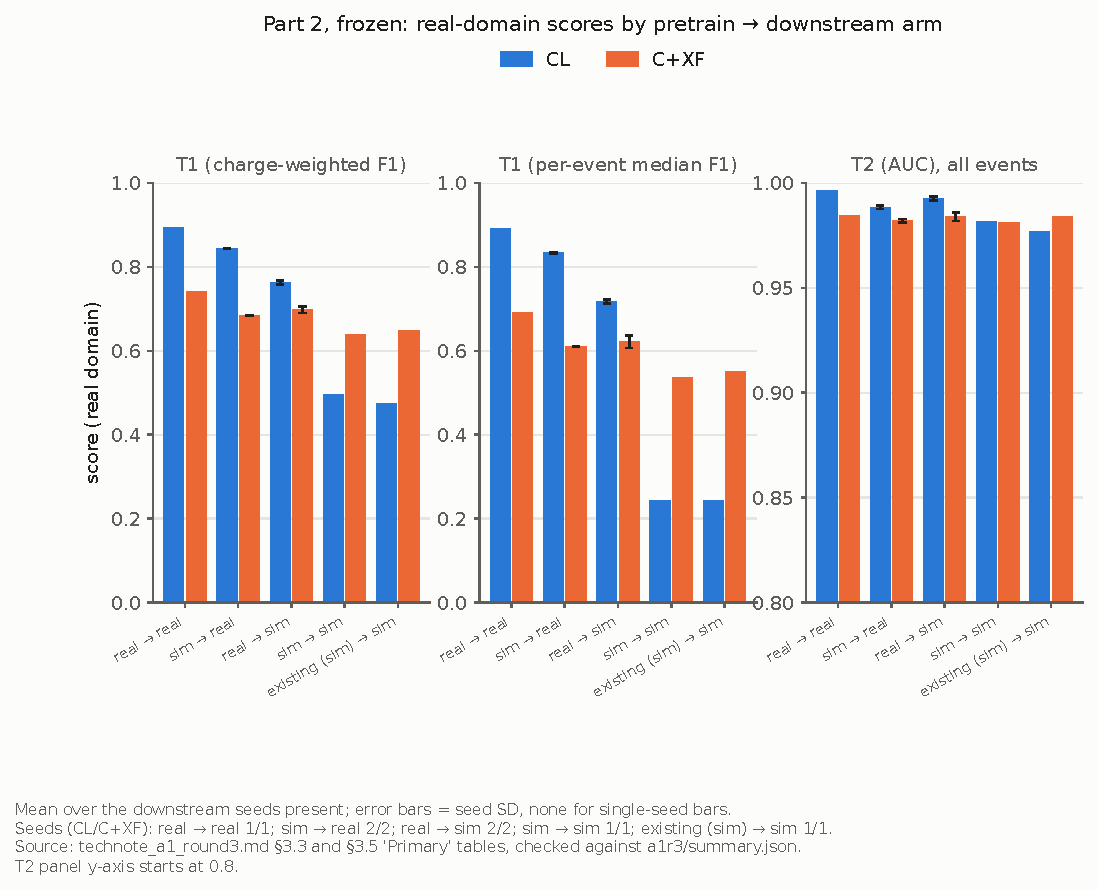
\includegraphics[width=0.92\linewidth,height=0.42\textheight,keepaspectratio]{a1r3_part2_frozen_primary.pdf}\caption{Part 2, frozen: real-domain T1 (charge-weighted and per-event median) and T2 (all events) by pretrain $\rightarrow$ downstream arm, for CL (§3.3) and C + XF (§3.5), 'Primary' tables. Mean $\pm$ seed SD over the seeds present; single-seed arms have no error bar.}\end{figure}
\subsection{Part 2 findings}
All comparisons are on the real domain unless stated otherwise.

\begin{enumerate}
\item \textbf{sim $\rightarrow$ real vs real $\rightarrow$ real (does pretraining domain matter when the downstream domain is real?).}
\begin{itemize}
\item \textbf{CL finetune:} the two are within 0.005. T1 charge-weighted 0.9214 against 0.9175 (single-seed control), and bright T2 0.9939 against 0.9934.
\item \textbf{CL frozen:} real pretraining helps, 0.893 against 0.845 ($-$0.049).
\item \textbf{C + XF:} sim pretraining costs 0.052 (finetune, 0.829 against 0.881) and 0.058 (frozen, 0.684 against 0.741). C + XF pretraining sees only the width shift, so this is the effect of a width-only domain mismatch in the backbone.
\item The decomposition tables show the real-domain gain over the sim domain is almost entirely from the widths.
\end{itemize}
\item \textbf{real $\rightarrow$ sim vs sim $\rightarrow$ sim (does pretraining domain matter when the downstream domain is sim?).} Both arms train downstream on sim. Real pretraining raises the real-domain T1 in every arm.
\begin{itemize}
\item \textbf{CL frozen:} real-domain T1 0.763 against 0.496 (+0.27). Its sim-domain T1 is 0.868 against 0.893.
\item \textbf{CL finetune:} 0.666 against 0.598 (+0.07); sim-domain T1 0.922 against 0.925.
\item \textbf{C + XF:} real-domain 0.808 against 0.767 (finetune) and 0.698 against 0.639 (frozen). In the sim domain, C + XF real $\rightarrow$ sim is better than sim $\rightarrow$ sim by 0.035 (finetune) and 0.047 (frozen).
\item Domain-robust features from real pretraining thus carry over to downstream heads trained on sim, but not as far as training downstream on real: no real $\rightarrow$ sim arm reaches the sim $\rightarrow$ real or real $\rightarrow$ real level.
\end{itemize}
\item \textbf{Frozen vs finetune.}
\begin{itemize}
\item Finetuning raises the real-domain T1 in every arm where the downstream domain is real, by 0.077 (CL sim $\rightarrow$ real, 0.845 $\rightarrow$ 0.921), 0.024 (CL real $\rightarrow$ real), 0.146 (C + XF sim $\rightarrow$ real) and 0.140 (C + XF real $\rightarrow$ real).
\item For real $\rightarrow$ sim, finetuning lowers CL (0.763 $\rightarrow$ 0.666) and leaves C + XF higher (0.698 $\rightarrow$ 0.808). Frozen CL real $\rightarrow$ sim reaches 0.763 on the real domain with no real downstream data, so a good part of the real-domain performance is carried by the pretrained features.
\end{itemize}
\item \textbf{CL vs C + XF.} CL is better when the downstream domain is real: finetuned real $\rightarrow$ real 0.9175 against 0.8813, sim $\rightarrow$ real 0.9214 against 0.8294. C + XF is less sensitive to the domain: existing $\rightarrow$ real costs 0.05 (against 0.30 for CL), so it ends higher than CL for sim-trained models (0.808 against 0.621).
\item \textbf{Where the real-domain loss comes from.} The width correction accounts for almost all of it. The light correction (\texttt{l\_\allowbreak{}comb80}) costs at most 0.022 in T1 (C + XF frozen, sim-downstream arms) and 0.006 or less for CL, as in the light round.
\item \textbf{\texttt{d\_\allowbreak{}real\_\allowbreak{}noVnorm} (link to Part 1).} Using the un-normalised V table in the real domain lowers every arm's T1 charge-weighted, by 0.09--0.21 for CL and 0.002--0.06 for C + XF. Even CL real $\rightarrow$ real falls from 0.9175 to 0.8102 (finetune) and from 0.8934 to 0.7291 (frozen). The real-domain scores above therefore depend on the V normalisation choice. For finetuned CL the two real-downstream arms stay well above the sim-downstream ones (0.81--0.83 against 0.47--0.52).
\item \textbf{Reproduction (new sim $\rightarrow$ sim vs existing models, sim domain).}
\begin{center}\footnotesize
\setlength{\tabcolsep}{3pt}\renewcommand{\arraystretch}{1.15}
\begin{tabularx}{\linewidth}{LLLLLL}
\toprule
\textbf{Model} & \textbf{Mode} & \textbf{Existing T1 cw} & \textbf{New sim $\rightarrow$ sim T1 cw} & \textbf{Existing T2 all} & \textbf{New T2 all} \\
\midrule
CL & finetune & 0.9185 $\pm$ 0.0002 & 0.9252 & 0.9932 $\pm$ 0.0028 & 0.9947 \\
CL & frozen & 0.8944 & 0.8932 & 0.9971 & 0.9963 \\
C + XF & finetune & 0.8593 $\pm$ 0.0017 & 0.8654 & 0.9899 $\pm$ 0.0005 & 0.9921 \\
C + XF & frozen & 0.7207 & 0.7136 & 0.9839 & 0.9811 \\
\bottomrule
\end{tabularx}
\end{center}
The disjoint pretrain/downstream split and re-pretraining change the sim-domain T1 by 0.001 to 0.007 and T2 by at most 0.003. The new sim $\rightarrow$ sim runs are single seeds, so the comparison is against the round-2 seed SD of about 0.002. These checks support the sim $\rightarrow$ sim control as a like-for-like partner of the real arms.
\end{enumerate}
\section{Caveats}
\begin{itemize}
\item \textbf{``Real'' is a modelled data-like domain,} built from the round-2 width factors and the \texttt{l\_\allowbreak{}comb80} light correction. It is not detector data. Widths are corrected on simulated-$\nu$ hits only; light on all ophits of flash events (sim ophits are not labelled).
\item \textbf{C + XF pretraining sees only the width part of the shift} (charge-only backbone). Its light correction acts only downstream and at evaluation.
\item \textbf{One pretraining seed per backbone.} Seed spread is downstream only, over two seeds per arm and one for controls. Quote bootstrap CIs, and do not read differences below about 0.01 in T1 without them.
\item \textbf{Rerun of two runs.} A job-queue lock race ran \texttt{cl\_\allowbreak{}sim2real\_\allowbreak{}finetune\_\allowbreak{}s1} and \texttt{cl\_\allowbreak{}real2sim\_\allowbreak{}finetune\_\allowbreak{}s0} twice concurrently each, interleaving their logs. Both were rerun on 2026-11-23 and the tables use the rerun results; the quarantined outputs are in \texttt{a1r3/\allowbreak{}quarantine\_\allowbreak{}race\_\allowbreak{}20261123/\allowbreak{}}. Real-domain T1 charge-weighted, old $\rightarrow$ new: 0.9219 $\rightarrow$ 0.9214 (\texttt{cl\_\allowbreak{}sim2real\_\allowbreak{}finetune\_\allowbreak{}s1}) and 0.6484 $\rightarrow$ 0.6681 (\texttt{cl\_\allowbreak{}real2sim\_\allowbreak{}finetune\_\allowbreak{}s0}).
\item \textbf{Energy and light test scores are not reported.} Only T1 and T2 are in scope, and the T5 targets stay native in the real-domain downstream runs.
\item \textbf{T2 bright} uses the native 3--6 $\mu$s PE $\geq$ 200 subset, not the paper \texttt{truth.npz} cut.
\item \textbf{Inference runs in bf16}, as in round 2 (irrelevant at these effect sizes).
\item \textbf{Stage 1a launch bug.} Only 3 of the 4 pretrains were launched in the first stage-1 job (fixed; the fourth ran in stage 1b). It affected the schedule, not the results.
\end{itemize}
\section{Compute and reproducibility}
\textbf{Jobs} (Polaris, 4 $\times$ A100 per node, account \texttt{LArTPC\_\allowbreak{}FM}). Walltime runs from the first start to completion, as logged in \texttt{a1r3/\allowbreak{}STATUS}, with requeues included.

\begin{center}\footnotesize
\setlength{\tabcolsep}{3pt}\renewcommand{\arraystretch}{1.15}
\begin{tabularx}{\linewidth}{LLLLLLL}
\toprule
\textbf{Stage} & \textbf{Job} & \textbf{Queue} & \textbf{Nodes} & \textbf{Walltime (h)} & \textbf{Node-hours} & \textbf{Notes} \\
\midrule
0 & 7862003 & debug & 2 & 0.35 & 0.70 & tests, splits, smoke, gates, Part 1 (6 runs) \\
1a & 7862258 & preemptable & 4 & 2.07 & 8.27 & 3 of 4 pretrains launched (launch bug, now fixed) \\
1b & 7869665 & preemptable & 4 & 4.69 & 18.74 & one remaining pretrain (\texttt{real\_\allowbreak{}c}), with requeues \\
2 & 7873432 & preemptable & 6 & 2.36 & 14.17 & 24 downstream runs, one requeue \\
3 & 7875850 & preemptable & 4 & 1.28 & 5.13 & 32 evaluations and summary \\
rerun, stage 2 & 7880513 & debug & 1 & 0.81 & 0.80 & the 2 raced downstream runs; 22/24 already done, still 22/24 at its end \\
rerun, stage 2 retry & 7880705 & debug & 1 & 0.30 & 0.30 & finished the 2 raced runs (24/24) \\
rerun, stage 3 & 7880812 & debug & 1 & 0.18 & 0.18 & 2 re-evaluations (30/32 already done) and summary \\
 &  &  &  & \textbf{total} & \textbf{$\approx$ 48.3} (47.0 + 1.28 rerun) &  \\
\bottomrule
\end{tabularx}
\end{center}
The plan expected $\approx$ 22 nh ($\approx$ 34 nh maximum charged). The overrun comes from preemptable requeues, the first-launch bug (stage 1a charged for 4 nodes with 3 pretrains), and holding a 4-node allocation for \texttt{real\_\allowbreak{}c} (a single-node run) through the stage 1b requeues.

Rerun (2026-11-23): submitted 17:09; stage 2 started 17:49 (debug queue wait 0.7 h), the retry 19:15, stage 3 20:24; summary complete 20:35. Node-hours are nodes $\times$ (end $-$ start) from the \texttt{job started} lines to the next stage submission or COMPLETE.

Queue waits per stage: stage 0, 1.7 h; stage 1a, 36 h; stage 1b, 16 h; stage 2, 11 h; stage 3, 11 h. The campaign took about 4 days from submission (2026-11-19 03:08) to the summary (2026-11-22 18:22).

Verification against \texttt{STATUS}: the stage 0 to 3 start and end times reproduce the walltimes and node-hours above. The \texttt{STATUS} file shows stage 1b with four starts (11:17, 11:39, 14:21, 15:35 on 2026-11-21), stage 2 with two (03:12 and 04:50 on 2026-11-22), and stage 3 with two (17:06 and 17:49 on 2026-11-22). The node-hours are wall from the first start and may overstate the charge if the preempted segments were shorter than the elapsed time.

\textbf{Code} (jpeterso copy): \texttt{qlfm/\allowbreak{}eval\_\allowbreak{}perturb.py} (\texttt{w\_\allowbreak{}meas3d\_\allowbreak{}noVnorm} variants, \texttt{--absolute-domain}, composite \texttt{d\_\allowbreak{}real} variants), \texttt{scripts/\allowbreak{}a1r3\_\allowbreak{}make\_\allowbreak{}splits.py}, round-3 stage scripts under \texttt{scripts/\allowbreak{}pbs/\allowbreak{}a1r3\_\allowbreak{}stage*.pbs}, and the summary generator that wrote \texttt{summary.md} and \texttt{summary.json}. Domain support in \texttt{train\_\allowbreak{}pretrain.py} and \texttt{train\_\allowbreak{}multitask.py} (\texttt{--domain sim|real}) and the per-run \texttt{event\_\allowbreak{}lists.npz} outputs.

\textbf{Inputs:} existing models in \texttt{/\allowbreak{}lus/\allowbreak{}eagle/\allowbreak{}projects/\allowbreak{}neutrinoGPU/\allowbreak{}yuhw/\allowbreak{}fm4npp-lartpc-work/\allowbreak{}s3/\allowbreak{}mt/\allowbreak{}qlfm\_\allowbreak{}M\_\allowbreak{}\{CL,C\_\allowbreak{}xf\}/\allowbreak{}}.

\appendix
\section{Per-seed real-domain values}
Seeds in the order listed.

\subsection{CL, finetune}
\begin{center}\footnotesize
\setlength{\tabcolsep}{3pt}\renewcommand{\arraystretch}{1.15}
\begin{tabularx}{\linewidth}{LLLLLL}
\toprule
\textbf{pretrain $\rightarrow$ downstream} & \textbf{seeds} & \textbf{T1 cw} & \textbf{T1 evt-median} & \textbf{T2 all} & \textbf{T2 bright} \\
\midrule
real $\rightarrow$ real & 0 & 0.9175 & 0.9203 & 0.9970 & 0.9934 \\
sim $\rightarrow$ real & 0, 1 & 0.9214, 0.9214 & 0.9242, 0.9241 & 0.9961, 0.9961 & 0.9949, 0.9930 \\
real $\rightarrow$ sim & 0, 1 & 0.6681, 0.6636 & 0.6209, 0.6230 & 0.9710, 0.9606 & 0.9594, 0.9571 \\
sim $\rightarrow$ sim & 0 & 0.5981 & 0.5213 & 0.9293 & 0.9002 \\
existing (sim) $\rightarrow$ sim & 0, 1, 2 & 0.6336, 0.6215, 0.6079 & 0.5853, 0.5744, 0.5529 & 0.9456, 0.9267, 0.9478 & 0.9360, 0.8915, 0.9131 \\
\bottomrule
\end{tabularx}
\end{center}
\subsection{CL, frozen}
\begin{center}\footnotesize
\setlength{\tabcolsep}{3pt}\renewcommand{\arraystretch}{1.15}
\begin{tabularx}{\linewidth}{LLLLLL}
\toprule
\textbf{pretrain $\rightarrow$ downstream} & \textbf{seeds} & \textbf{T1 cw} & \textbf{T1 evt-median} & \textbf{T2 all} & \textbf{T2 bright} \\
\midrule
real $\rightarrow$ real & 0 & 0.8934 & 0.8920 & 0.9964 & 0.9882 \\
sim $\rightarrow$ real & 0, 1 & 0.8442, 0.8453 & 0.8330, 0.8349 & 0.9880, 0.9892 & 0.9575, 0.9630 \\
real $\rightarrow$ sim & 0, 1 & 0.7594, 0.7658 & 0.7138, 0.7213 & 0.9922, 0.9935 & 0.9680, 0.9737 \\
sim $\rightarrow$ sim & 0 & 0.4958 & 0.2434 & 0.9818 & 0.9471 \\
existing (sim) $\rightarrow$ sim & 0 & 0.4736 & 0.2431 & 0.9770 & 0.9363 \\
\bottomrule
\end{tabularx}
\end{center}
\subsection{C + XF, finetune}
\begin{center}\footnotesize
\setlength{\tabcolsep}{3pt}\renewcommand{\arraystretch}{1.15}
\begin{tabularx}{\linewidth}{LLLLLL}
\toprule
\textbf{pretrain $\rightarrow$ downstream} & \textbf{seeds} & \textbf{T1 cw} & \textbf{T1 evt-median} & \textbf{T2 all} & \textbf{T2 bright} \\
\midrule
real $\rightarrow$ real & 0 & 0.8813 & 0.8880 & 0.9833 & 0.9633 \\
sim $\rightarrow$ real & 0, 1 & 0.8249, 0.8339 & 0.8155, 0.8291 & 0.9864, 0.9847 & 0.9604, 0.9532 \\
real $\rightarrow$ sim & 0, 1 & 0.8021, 0.8131 & 0.7871, 0.8090 & 0.9798, 0.9809 & 0.9505, 0.9537 \\
sim $\rightarrow$ sim & 0 & 0.7667 & 0.7298 & 0.9847 & 0.9565 \\
existing (sim) $\rightarrow$ sim & 0, 1, 2 & 0.8082, 0.8105, 0.8067 & 0.7910, 0.7924, 0.7871 & 0.9863, 0.9870, 0.9861 & 0.9612, 0.9607, 0.9594 \\
\bottomrule
\end{tabularx}
\end{center}
\subsection{C + XF, frozen}
\begin{center}\footnotesize
\setlength{\tabcolsep}{3pt}\renewcommand{\arraystretch}{1.15}
\begin{tabularx}{\linewidth}{LLLLLL}
\toprule
\textbf{pretrain $\rightarrow$ downstream} & \textbf{seeds} & \textbf{T1 cw} & \textbf{T1 evt-median} & \textbf{T2 all} & \textbf{T2 bright} \\
\midrule
real $\rightarrow$ real & 0 & 0.7413 & 0.6903 & 0.9845 & 0.9484 \\
sim $\rightarrow$ real & 0, 1 & 0.6831, 0.6840 & 0.6098, 0.6103 & 0.9827, 0.9815 & 0.9359, 0.9320 \\
real $\rightarrow$ sim & 0, 1 & 0.6929, 0.7037 & 0.6111, 0.6323 & 0.9826, 0.9854 & 0.9506, 0.9528 \\
sim $\rightarrow$ sim & 0 & 0.6385 & 0.5361 & 0.9814 & 0.9367 \\
existing (sim) $\rightarrow$ sim & 0 & 0.6486 & 0.5506 & 0.9843 & 0.9461 \\
\bottomrule
\end{tabularx}
\end{center}
\end{document}
